%!TEX root = thesis.tex
As we noted in the introduction, the domestic environment is a domain where we find the relationship between computers and user interesting.
The domestic environment is interesting because we see the home as a space where adaptability, personalization, and ??  are central aspects of making a home \emph{home} and as such our idea of AHI, that we will present in chapter~\ref{ch:adhoc}, feels appropriate and relevant in this domain.
We have chosen this as a design constraint with the hope it will enable us to make a more precise and sharp presentation and exploration of the possibilities of AHIs as we are now forced to put it into a specific context.

As a point of origin we will first look at the building as a concept and how the building relates to changes and to the people that inhabits its walls.
Secondly we will look into so called ``smart homes'', homes where computers becomes large part of the ecology of the home, as this poses interesting possibilities and challenges for designing computer systems.

\section{The evolution of buildings}
Buildings, like everything else, changes over time.
But different parts of a building change with different rates, a wall will most likely endure longer than the paint on its sides and the ground on which the wall stands will most likely still be there when the wall collapses.
This ever changing nature of buildings has been conceptualized by Steward Brand in his book \emph{How Buildings Learn: What Happens After They're Built} \citep{brand1995buildings}.
Here Brand presents a framework, in which he define six S's as a ground for understanding changes in a building: Site, Structure, Skin, Services, Space plan and Stuff.

\begin{figure}[h]
	\centering
  		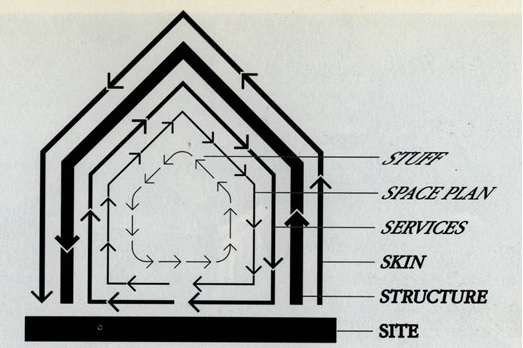
\includegraphics[width=3.5in]{figures/brand-diagram}
	\caption{The different layers of change \citep[chapter 2]{brand1995buildings}}
   \label{brand-diagram}
\end{figure}

The six S's describes the different layers of change, three describing the exterior: Site, Structure and Skin and three describing the interior: Services, Space plan and Stuff.
Each layer has a different rate of change, Site having the longest and Stuff the shortest rate of change, see figure~\ref{brand-diagram}.
As the rate of change differs for the different components of the building, the building is, as Brand notes, constantly `tearing itself apart', or in a more constructive term, constantly evolving.

Brand argues in favor for an approach where the inhabitants of a building can evolve and change the building over time according to their needs \citep{brandBBCvideo}.
He sees this in contrast to a scenario where a single person or group designs a building for others to use.
In light of this, providing inhabitants with higher rates of change could accommodate an even more dynamic relationship between the building and the people living in it.

We see two interesting ways of exploring this existing relationship between building and inhabitants.
One is to open up the layer of Stuff.
The layer of Stuff is all the things that gets moved around or changed on daily to monthly basis such as chairs and desks, kitchen appliances and lamps.
So what if Stuff could be changed, moved or modified on an even more frequent basis, say in minutes or hours, accommodating the need of the inhabitants with the possibility for them to adapt furniture and objects to current needs.

Another approach could be to pull down a given layer of change to a lower layer, for example enabling changes in the Space Plan as if it was Stuff, creating a more dynamic Space Plan.
This would open up for entirely new possibilities of rethinking the home. 
If, for example, homes had dynamic walls, ceilings, floors and doors that would give them a less static and permanent function, it could enable changes to the Space Plan that maybe lasts days or months, enabling the Space Plan to adapt to specific situations, just as you on the Stuff plan would add an extra chair to the table for a visiting guest. 

It is, of course, non trivial to make the home as dynamic and adaptable as suggested above.
But the this concept of the building as a living, ever-evolving entity, does give us inspiration to explore the use of digital systems in a domestic setting, as this could be one way to approach such a vision.
So with the help of computers and new materials we want to explore how we can accommodate and design for change in physical environment that surrounds us.
We want to explore how physical interfaces can be created on demand in an ad hoc manner, to better cope with the changes in the buildings space plan and on the level of stuff, and better accommodate the changing needs of its inhabitants.
As touched upon in chapter~\ref{ch:ui} this does somewhat challenge the traditional view of physical interfaces as they are generally considered static and permanent.
\todo{bedre afrunding til smart homes}
hvad skal der komme ud af det

Smart homes - ideen om det teknologiske hus
intro
definition/vision
complex setting
rodden - hvem skal deltage 

\section{Smart homes or home that make us smart}
\todo{section not done - needs work}

The idea of adding computer systems into the domestic environment is not a new one.
Ever since the emergence of electricity into the households, electrical appliances has been a part of the domestic setting.
And along with the increasingly more advanced appliances being developed, the dream and vision of even more sophisticated systems have continuously evolved

An early visual example of the fascination of `smart homes' is seen in the General Motors commercial film \emph{Design for Dreaming}\footnote{http://en.wikipedia.org/wiki/Design\_for\_Dreaming} from 1956 \citep{designfordreaming}, where the \emph{Home of the Future}\footnote{http://en.wikipedia.org/wiki/Home\_of\_the\_future} is presented.
Here we see a remote control of the different kitchen appliances, a (computer)screen that can show the final result of the recipe it is given, and a seemingly context-aware moving table.
Domestic technology appears even earlier where in the 1915-20, with the advent of electricity in common homes, electrically powered machines such as vacuum cleaners and refrigerators providing the `seedbed', as \citet{aldrich2003smart} puts it, for the emergence of the smart home.

In recent years, especially since Mark Weiser's vision of ubiquitous computing \citep{weiser1991computer}, a lot of the research in the domestic realm has focused on the idea of a \emph{home that is smart} where the goal is to use computers to make the home \emph{intelligent} \citep{taylor2007homes}.
\citet{aldrich2003smart} defines smart homes as:

\begin{quotation}
\emph{A ``smart home'' can be defined as a residence equipped with computing and information technology which anticipates and responds to the needs of the occupants, working to promote their comfort, convenience, security and entertainment through the management of technology within the home and connections to the world beyond.}
\end{quotation}
\citeauthor{aldrich2003smart} sees this definition as the acme of domestic technology as we can envision it today, putting it somewhere in between reality and fantasy.
\todo{mere her}

The domestic setting differs a lot from the traditional office setting where most research on ubiquitous computing has been conducted, and is in some ways even more complex as people in the domestic setting has a lot more freedom as to how they organize their space and time \cite{meyer2003survey}.
Also the aspect of user experience needs special consideration when introducing new technology to the home, whereas in a work setting the user might \emph{need} to use the new technology, imposed upon him by superiors, the technology for the home need to be usable and useful enough so that the user \emph{wants} to use \citep{meyer2003survey}.
\todo{maaske undlade naeste del}
A thorough look at the challenges related to creating ubiquitous computing for the home is presented by \citet{edwards2001home}.
Here Edwards et al. identifies seven challenges that need to be overcome before the vision of the ubiquitous smart home can become a reality. We will return to these challenges in relation to our own prototypes \todo{ref til prototype sektion}.

\citet{rodden2003evolution} have built upon Brands framework in the context of ubiquitous computing and the domestic setting and is therefore relevant for us here.
By looking at existing research Rodden et al. identifies three main approaches for creating interactive devices for domestic settings.

\begin{itemize}
  \item \emph{Information Appliance} that are stand-alone, self-contained devices that are often used as a layer of interactive functions on top of an existing appliance.
  \item \emph{Interactive Household Objects} that embeds interactive capabilities into existing household objects to create new means of interaction and communication, often building upon the existing understanding and metaphors associated with the household object.
  \item \emph{Augmented Furniture} that embeds sensory systems into furniture to add interactive capabilities. \ldots
\end{itemize}

Rodden et al. notes that the technology is most intrusive in information appliances, less so in interactive household objects and least in augmented furniture.

\todo{noget om bygninger ikke er nybyggerier og noget mere Rodden}
 
\todo{diskussion om empoverment, Brand/Rodden vs smart-homes/context-awareness/dubai-huse}

\todo{make systems that are not dictated by a designer, but made for adaptation and modification. People are different and have different, changing, needs. Systems needs to repsond to this}
